\begin{figure}
  \setlength{\unitlength}{\textwidth}

        \begin{picture}(1,0.3)(0.0,0.45)

      % % % Parkinson Data 
      \put(0.025,0.5){\includegraphics[width=0.5\unitlength]{../FnP/gnuplot/mean_power_collapsed_mstar_175.eps}}      \put(0.495,0.5){\includegraphics[width=0.5\unitlength]{../FnP/gnuplot/mean_power_collapsed_parkinson_10.eps}}
      
      \put(0.23,0.48){ $\displaystyle\frac{c}{\rho\mathcal{A}U}$}
      \put(0.73,0.48){ $\displaystyle\frac{c}{\rho\mathcal{A}U}$}
          
      \put(0.0,0.63){\large$\frac{P_{m}}{\rho \mathcal{A}U^3 }$}
      
      \put(0.085,0.709){\small(a)}
      \put(0.555,0.709){\small(b)}
     
      
    \end{picture}
  \caption{Mean power as a function of damping factor. Data presented in both (a) and (b) were calculated using input data at \reynoldsnumber=22300 \cite{Parkinson1964} where (a) shows mean power data at six different mass ratios:$m^*=1$ ($\times$), $m^*=5$ (\ding{110}), $m^*=10$ (+), $m^*=50$ (\ding{108})), $m^*=100$ (\ding{116}) and $m^*=1164$ (\ding{83}) at \ustar=175. Data presented in (b) shows mean power data at three different reduced velocities: \ustar=75 (\ding{108}), \ustar=175 (\ding{116}) and \ustar=375 (\ding{83}) at $m^*=10$. The maximum mean power tend to increase with decreasing $m^*$ as well as increasing \ustar at low $m^*$. }  
    
    \label{fig:mstarcollapsed_parkinson}
\end{figure}

\ %vspace{10cm}
